%------------------------------------------------
\section{Ускорительные комплексы}

\begin{frame}
	
	\frametitle{Открытия частиц}
	\begin{table}[h!]
		\tiny
		\begin{longtable}{|p{3cm}|p{2cm}|p{3cm}|p{5cm}|}
			\hline
			\textbf{Частица} & \textbf{Год открытия} & \textbf{Ускоритель} & \textbf{Значение открытия} \\
			\hline
			
			\hline
			Бозон Хиггса & 2012 & LHC (CERN) & Завершение Стандартной модели, объяснение механизма массы элементарных частиц \\
			Топ-кварк & 1995 & Tevatron (Fermilab) & Последний предсказанный кварк, подтверждение кварковой модели \\
			W и Z бозоны & 1983 & SPS (CERN) & Подтверждение электрослабого взаимодействия, Нобелевская премия 1984 \\
			Глюон & 1979 & PETRA (DESY) & Экспериментальное подтверждение существования переносчика сильного взаимодействия \\
			Антисигма-минус гиперон ($\bar{\Sigma}^-$) & 1975 & Синхрофазотрон (ОИЯИ, Дубна) & Обнаружение античастицы гиперона \(\Sigma^-\), важное открытие для понимания свойств антиматерии и странных частиц \\
			Очарованный кварк ($J/\psi$ мезон) & 1974 & SLAC / BNL & Начало «революции очарования», подтверждение существования четвертого кварка \\
			Антипротон ($\bar{p}$) & 1955 & Bevatron (Berkeley) & Подтверждение предсказанной Дираком антиматерии, ключ к физике частиц \\
			Каоны ($K^\pm, K^0$) & 1947 & Космические лучи, Bevatron & Доказательство существования странных частиц, начало изучения CP-нарушения \\
			Пион ($\pi^\pm, \pi^0$) & 1947 & Космические лучи, Bevatron & Первое экспериментальное подтверждение мезонов, предсказанных Юкавой \\
			\hline
		\end{longtable}
	\end{table}
\end{frame}

\begin{frame}
	\frametitle{Современные ускорительные центры}
	
		\begin{table}[h!]
			\tiny
		\begin{tabular}{|p{1.3cm}|p{1cm}|p{2cm}|p{1.5cm}|p{2cm}|p{4cm}|}
			
			\hline
			\textbf{Название} & \textbf{Страна} & \textbf{Тип ускорителя} & \textbf{Энергия} & \textbf{Основные эксперименты} & \textbf{Основные исследования} \\
			\hline
			
			\hline
			LHC (CERN) & Швейцария / Франция & Кольцевой коллайдер (pp, Pb-Pb) & 6.8 ТэВ (на пучок) & ATLAS, CMS, ALICE, LHCb & Бозон Хиггса, кварк-глюонная плазма, новая физика \\
			RHIC (BNL) & США & Кольцевой коллайдер (Au-Au, p-p) & 100 ГэВ/нуклон & STAR, PHENIX & Фазовый переход в кварк-глюонную плазму, спиновые структуры \\
			NICA (ОИЯИ, Дубна) & Россия & Кольцевой коллайдер (Au-Au) & 11 ГэВ/нуклон & MPD, SPD & Плотная барионная материя, критическая точка фазового перехода \\
			FAIR (GSI) & Германия & Кольцевой и линейные ускорители & 35 ГэВ/нуклон & CBM, HADES, PANDA, COSY & Адроны, экзотические состояния материи, антиядра \\
			SuperKEKB (KEK) & Япония & Кольцевой коллайдер (e⁺e⁻) & 7 ГэВ (e⁺) + 4 ГэВ (e⁻) & Belle II & CP-нарушение, редкие распады B-мезонов \\
			J-PARC & Япония & Протонный ускорительный комплекс & 30 ГэВ & T2K, g-2/EDM & Осцилляции нейтрино, аномальный магнитный момент мюона \\
			CEPC (проект) & Китай & Будущий электрон-позитронный коллайдер (e⁺e⁻) & 120 ГэВ & - & Физика бозона Хиггса, поиск новой физики \\
			European XFEL (DESY) & Германия & Линейный рентгеновский лазер & 17.5 ГэВ (e⁻) & SPB, SCS & Ультрабыстрая динамика атомов, биология, наноматериалы \\
			\hline
		\end{tabular}
		\end{table}
	
\end{frame}


\begin{frame}
	\frametitle{Ускорительные комплексы. CERN}

	\begin{figure}
		\centering
		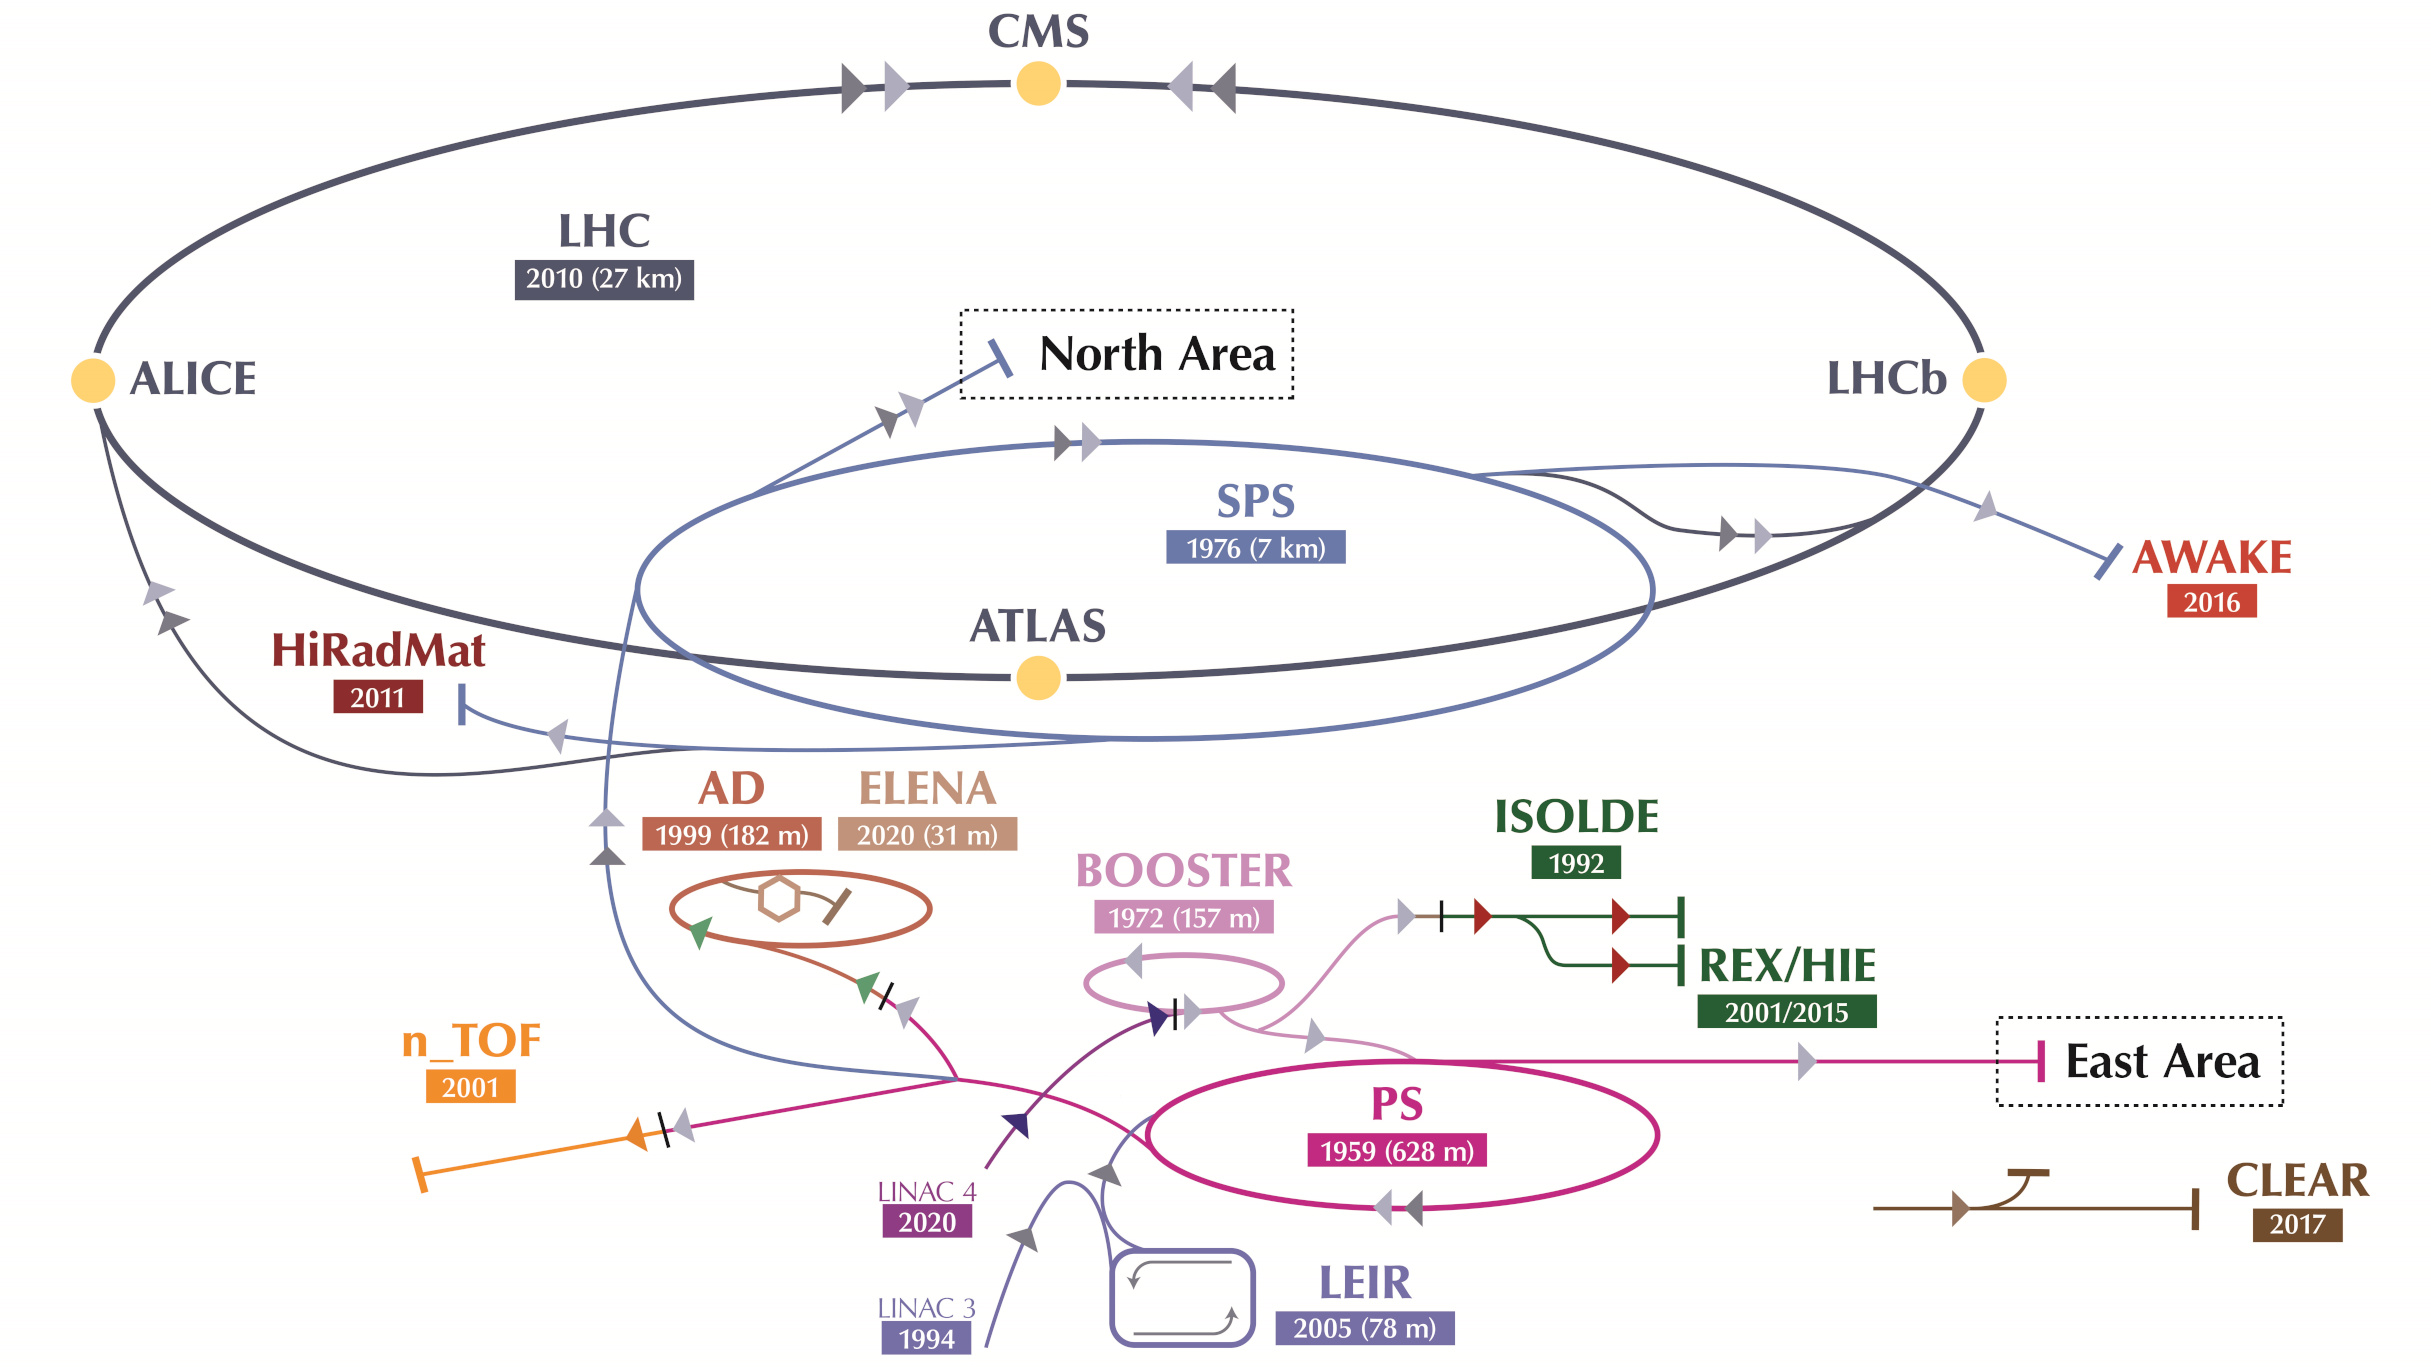
\includegraphics[width=0.7\linewidth]{images/cern-complex}
	\end{figure}
	
\end{frame}


%------------------------------------------------